\documentclass{llncs}

\usepackage{llncsdoc}
\usepackage{hyperref}
\usepackage{url}
\usepackage{graphics, graphicx}
\usepackage{caption}
\usepackage{csquotes}


\title{A Statistical Analysis of Adaptive Hints}

\author{Zhen Zhai\inst{1} \and Yoav Freund\inst{2}}
\institute{UC San Diego \email{zzhai@eng.ucsd.edu} \and UC San Diego \email{yfreund@eng.ucsd.edu}}



\begin{document}

\maketitle


%%%%%%%%%%%%%%%%%%%%%%%%%%%%%%%%%%%%%%%%%%%%%%%%%%%%%%%%%%%%%%%%%%%%%%%%%%%%%%%%
\begin{abstract}
We propose an adaptive hint system for mathematical homework assignment. Some of the hints are generic and are triggered by universal triggers. Other hints are problem specific and are created by the teaching staff ahead of time. The number of possible answers after receiving the hints is still very large, which makes it hard for students to game the system.

We describe a deployment of our system in an undergraduate course in probability and statistics involving 300 students. We present an analysis of the logs from the deployment and show that exposure to hints reduced the number of attempts and the amount of time spent in the attempts for {\em questions without hints that were answered after the question with the hint}. Demonstrating that the hints had a long term positive effect on the performance of the students. On the other hand, there was no significant correlation between the reception of hints and the performance of the students in the final exam.

\end{abstract}


%%%%%%%%%%%%%%%%%%%%%%%%%%%%%%%%%%%%%%%%%%%%%%%%%%%%%%%%%%%%%%%%%%%%%%%%%%%%%%%%
\section{Introduction}
Intelligent tutoring systems (ITS)\cite{Anderson1995} attempt to replicate the interaction between a human tutor and a student. The goal is to detect and classify student errors and to provide instantaneous feedback to help students correct their error, but without "feeding" them the correct answer. Previous research suggests that a computer tutor can nearly be as effective as a human tutor\cite{Vanlehn2011}. Hence, many intelligent tutors have been developed and introduced into classrooms. A few well developed ITS designed for algebra curriculum in middle school and high school mathematics has already been proven to be effective\cite{Koedinger1997,John2014}.

Research has suggested that well-designed feedback is essential to improving the learning process\cite{Azevedo1995}\cite{Bangert-Drowns1991}. We target formative feedback as our hints to students. Formative feedback is feedback that aim to improve students learning, and is presented in the form of a response to student incorrect answers\cite{Shute2008}. According to Shute~\cite{Shute2008}, formative feedback needs to be specific, clear and timely. Furthermore, formative feedback should provide learners with both verification and elaboration\cite{Mason2001}\cite{Bangert-Drowns1991}. Verification is to provide feedback to learners as to whether the answer is correct or not. Elaboration is to provide a short elaboration on the topic or discuss the learner's incorrect answer. The timing of the feedback is important as well, we used delayed feedback supported by Kulhavy and Anderson's research\cite{Kulhavy1972}. We delay our hints by only providing hints to students who have spent a certain amount time on the problem without solving it. This allow the hints only go to students who are struggling on a problem. Finally, studies show that hint-on-demand allow students to learn more as compared to proactive hints\cite{Razzaq2010}. Therefore, our system is designed that a student will only see a hint if they click the 'Show Hint' button.

Homework is an essential part of students' learning process\cite{Cooper2006}. It gives students a chance to practice. Even more importantly, it allows them to identify their confusions and resolve them. There are many popular web-based homework systems for college students(e.g., WebAssign, WebWork, OWL, Andes). The goal is to help instructors to have a better management of a large enrollment class. These homework systems often provide feedback to students and provide analysis of student performance to instructors. Research has proven the web-based homework(WBH) systems to be helpful in learning\cite{MestHartRath2002}\cite{Vanlehn2005}. In these studies, the WBH systems, OWL and Andes, provide students with immediate feedback and hints following an incorrect attempt\cite{MestHartRath2002}\cite{Vanlehn2005}. The feedback and hints are the essential part of a WBH system, which is what our study focus on.

In~\cite{ElkherjFreund14} we described a system for delivering hints in the context of a web-based homework system. In the work presented here we describe a controlled experiment that we have done in the context of an undergraduate course in probability and statistics. Our statical analysis provides new evidence that adaptive hints are effective.

There is a common concern about students gaming the system, especially on harmful gaming, where gaming the system leads to poor learning outcome\cite{Baker2004}\cite{Baker2005}. In previous studies, students game the system by tricking the tutoring systems into giving out correct answers\cite{Baker2004Off-task}. As a result, students succeed in homework but fail on learning. We don't have this concern because our hints don't contain correct answers in any form. The adaptive hint system generates short simple questions as hints instead of worked-examples, which is commonly used among human tutors\cite{Atkinson2000}. In fact, it is suggested that worked examples have no significant effects on learning in a web-based intelligent tutoring environment\cite{McLaren2006}. Therefore, we replaced worked examples with short questions that are designed to promote thinking and guide student's learning process. This resolve the concern of students gaming the system because our system gives students hints on how to learn instead of how to answer a specific question. The only way for a student to obtain correct answers is by learning how to solve the problem. Therefore, we not only prevent any system gaming, but our hints also help students in long term. Furthermore, our hint system targets mathematic problems, which require students to type in mathematic expressions. Therefore, unlike multiple choice problems, it would be nearly impossible to guess the answer by looking at hints. There is infinity many ways one can type in a mathematic expression and it is very hard for students to simply guess it correctly with the help of hints. Therefore, we don't have the concern of students gaming the system.

\subsection*{Contribution}
We built and implemented an adaptive hint system to provide hints to students at the time they are struggling with homework. The adaptive hint system first studies a student's incorrect answer to identify the student's confusion. We target mathematic problems that require students to type in a expression, therefore the system generates a message to point out the incorrect subexpression in a student's answer. Then, based on the identified confusion, the system explains the identified confusion with a short sentence follow by a short question for the student to solve. This short question is specifically designed to target the student's confusion and it is simple enough that a student can easily understand and answer. Our goal is to let the student solve the smaller task before moving on to solve the bigger task. The goal of the adaptive hint system is to guides students in their learning process from understanding their confusions to resolve their confusions.

The system is adopted in a probability and statistic class of around 300 students and 245 students participated in this research. Each week we assign one assignment to students and we sent hints from the fourth week to the eighth week of the quarter. There are a total of 26 problems and each problem has between 1 to 10 questions. According to our record, students have received a total of 3621 hints during these five weeks. Our statistical result shows that students, with the help of the adaptive hints, learn to solve the problem and can solve similar problems more efficiently afterward. Our analysis demonstrates with statistical significant $p=0.029$ and $p=0.012$ that students who view the hints spent on average 14 less attempts and 26 minutes less on later problems in the same assignment comparing to students who didn't see the hints.


\section{The Adaptive Hint System}
The adaptive hint system is built on top of Open edX, an open source MOOC platform. We used Open edX as our homework system and embedded our adaptive hint system on top of Open edX. The edX homework system prompts students to answer problems by entering mathematical expressions and provides instant feedback on the correctness of the answer. The adaptive hint system provides additional feedback in the form of a hint. Students receive one assignment per week. Each assignment contains 5 to 10 problems and each problem has 1 to 10 parts. The problems in an assignment all target similar material that is covered in lecture. Students have an unlimited number of attempts for each problem, they can spend as many attempts as they want until they get to the correct answer.

Our adaptive hint system is built by creating hints ahead of time based on historical data. After we release the homework, the hint system starts to parse student attempts to figure out students' confusion. Then it looks for the appropriate hint in the hint database and sends to students.

\subsection*{Creating Hints}

Hints are created before we release the homework assignments. This allows the system to have a pool of hints to start with at the time the assignment is released. To create useful hints, the teaching staff analyzes the incorrect student attempts from previous quarters and create hints accordingly. The hints created are consist of a short explanation followed by a short question for the student to answer.

For example, one question would be "How many strings contain $k$ digits and $j$ uppercase letters?". The correct answer is $10^k*26^j*C(k+j,k)$. Suppose a student answers $10^k*26^j*(k+j)!$, the system would identify the incorrect subexpression and generate the following hint

\begin{displayquote}
The subexpression $10^k*26^j$ is correct, but not $(k+j)!$. How many ways are there to arrange 2 digits and 1 letter?
\end{displayquote}


This way we encourage students to focus on the incorrect part of their answers and solve a simpler version of it before attempting to solve the original problem. Moreover, as the hint is given in the form of a question, we guide the student to  think about the same problem in a simplified setting and leave it to them to infer the correct answer to the original problem. Note that students can choose to answer or not answer these hint questions. If students choose to answer the hint questions, we will provide instant feedback to let the students know whether their answers are correct or not. If students choose not to answer the hint questions, it won't hurt their grade.

Other than the problem specific hints, we also have generic hints. For example, when a student types in a number instead of an expression, our system will send a hint telling the student to type in an expression instead of the calculated result. Another example would be a hint pointing out that the question is asking for a positive number but the student typed in a negative number. These generic hints are designed to point out some very general mistakes students tend to make in a probability and statistics class. The system tends to send the generic hint before sending the specific hint.


\subsection*{Parse Trees}
The adaptive hint system needs to parse student attempts. Since we are targeting math expression problems, we can use parse trees to parse the math expressions. The parse tree always has operators as tree parents and operands as children. See Fig. \ref{fig:parse_tree}. Each tree node is marked by its position in the tree. The root node is node $R$. The left child node is indicated by $0$ and right child is $1$. Therefore, the left tree node of node $R$ is $R.0$, and right node is $R.1$. 

\begin{figure}[ht]
   \centering
   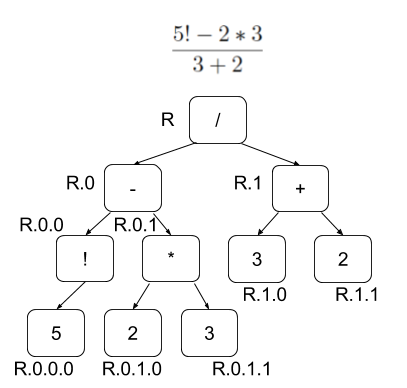
\includegraphics[width=.5\textwidth]{image/Parse_Trees.png}
   \caption{The parse tree mark each tree node by position. "R" stands for root node, "0" stands for left child node and "1" stands for right child node. Therefore, "R.0.1" stands for the right child node of the root's left child.}
   \label{fig:parse_tree}
\end{figure}

To figure out the mistake in an attempt, we compare the parse tree of the attempt with the parse tree of the correct answer. The tree comparison can tell us the subexpression that students make mistakes on. We can then classify student inputs based on the incorrect subexpressions and assign hints correspondingly. For example, the student who typed $5!-2*3$ and the student who typed $\frac{5!-2*3}{10}$ for a problem with solution $\frac{5!-2*3}{3+2}$, as in Fig. \ref{fig:parse_tree}, would be classified as the same group. Both of the students will have a mismatch of tree node $R.1$. This tells the system that the subtree of $R.1$ is wrong and the system will look for the corresponding hint.

One problem is that there are many different ways to write the same math expression. For example, $5!$ can also be written as $5*4*3*2*1$ or $5*4*3*2$. Therefore, we evaluate each subtree to a numerical result and use it in our comparison. The parse trees are evaluated bottom up. The operators at the bottom of the trees are evaluated first. The root operator is evaluated last. See Fig. \ref{fig:eval_tree}. 

\begin{figure}[ht]
   \centering
   \caption{The parse tree is evaluated bottom up. We first evaluate the lowest level of the tree then pass the evaluated results to the upper level. Then use the lower level results to evaluate the upper level of the tree until we reach the top node of the tree, the root, which will give us the final numerical result of the expression.}
   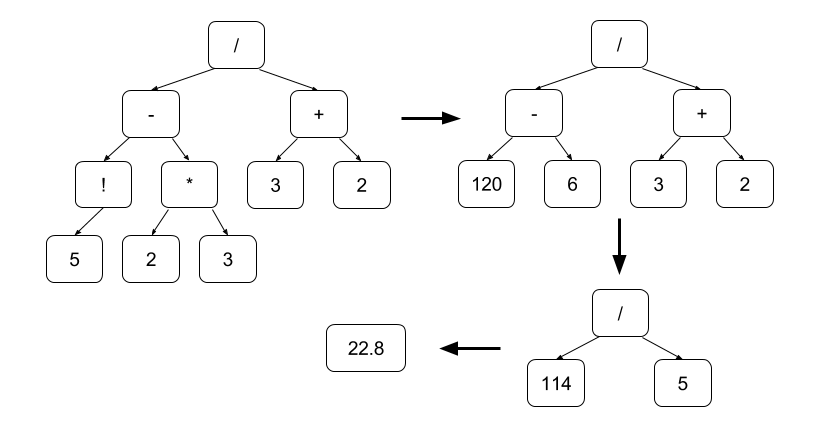
\includegraphics[width=0.8\textwidth]{image/Eval_Trees.png}
   \label{fig:eval_tree}
\end{figure}

Both the parse tree and the evaluation tree are used when we compare the attempt to the correct answer. We identify a subtree as incorrect only when neither of the evaluation and the subtree doesn't match. Therefore, $5!$ and $5*4*3*2*1$ will be identified as the same subtree because it evaluates to the same result.


\subsection*{Assigning Hints}
When TAs create hints, they are also asked to specify rules. Hint rules tell the system when to send certain hints and who the hints will go to. One example of hint rule for expression in Fig. \ref{fig:parse_tree} could be "$R.0.0$ is wrong" and the corresponding hint could be "You need to find the number of ways to arrange different poker cards. How many ways can you arrange 2 different cards?". When the hint system captures an attempt with an incorrect $R.0.0$ subtree, this hint will be sent. Such attempts could be $\frac{4!-2*3}{3+2}$ or $\frac{30-2*3}{3+2}$. The adaptive hint system will assign hints automatically based on the hint rules. This allows our hints to be sent automatically.

Note that the system doesn't send hints to student right away. Hints are only sent to students who have been working on the problem for more than 5 minutes or students who did more than 3 attempts. This is how the system send delayed hint suggested by Kulhavy and Anderson\cite{Kulhavy1972}. This way hints only go to students who are working on the problem actively and are struggling. Furthermore, students need to demand for hints by clicking the "Show Hints" button. Hint-on-demand is suggested to be more effective than proactive hints\cite{Razzaq2010}. Once a hint is assigned to a student, the student can choose to click or not click the "Show Hint" button. One can ignore the assigned hint by not clicking the "Show Hint" button. If a student wants to see the assigned hint, he/she needs to click the "Show Hint" button to see the hint. See Fig. \ref{fig:show_hint} In other words, we only show hints to students who ask for hints. Students who don't click the "Show Hints" button will not see the assigned hints. This makes sure we give on-demand hints to students who need helps and actively ask for help. 

\begin{figure}[ht]
   \centering
   \caption{First the system decides whether to assign hints to a student. Then the system search through the hint database to see whether there is a hint condition satisfied. Finally, the student gets to decide whether to see the assigned hint. A student will see a hint only if the system decides to assign the hint, a hint condition is satisfied, and the student clicked the ``Show Hint'' button.}
   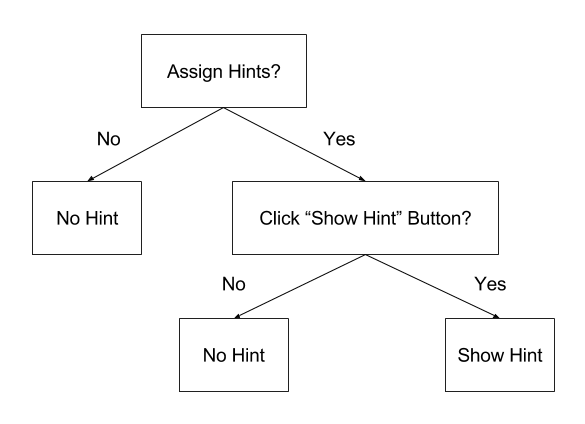
\includegraphics[width=0.7\textwidth]{image/Show_Hint.png}
   \label{fig:show_hint}
\end{figure}


\section{Statistical Study of the Effectiveness of hints}
%The hint system has recorded all the student attempts and the timestamps of each attempt. This allows us to extract useful features, including the number of attempts on each problem, time spent on each problem, etc. These features are used to study what effects hints make on students behavior.

We used a controlled study to quantify the effectiveness of our hint system. For each assignment, we randomly split the students into case and control with 50/50 chance. Case students will be able to receive hints on problems in the assignment, while control students will not receive any hint in the assignment. When a hint is assigned to a case student, one can choose whether or not to see the hint using the "Show Hint" button. Also, when a case student's attempt doesn't satisfy any of the hint rule, no hint will be sent. Therefore, for each problem in the assignment, we further filter out case students who received hints but didn't click 'Show Hint' and case students who received no hint because none of the hint condition is satisfied. We only focus on case students who actually received and saw the hint content. In other words, problems in each assignment will share the same group of control students but each problem will have a unique group of case students, which would be a subset of the case students of the assignment.

\subsection{Effect on Problems with Hint}
We first look at problems with hint. These problems have at least one hint sent out to at least one student. For each of the problem, we extract the number of attempts each student spent. We calculate the number of attempts average over case students and also the number of attempts average over control students. We compare these two numbers for each problem and found that control students spent fewer attempts on a problem compared to case students. See the left graph in Fig. \ref{fig:tries_times_analysis}. This shows that case students who clicked 'Show Hints' are the students who struggle with these problems and therefore spent more tries on the problems.

We also extract the time students spent on each problem. First we measured the time differences between each attempt and filtered those that are longer than 10 minutes. Time gaps larger than 10 minutes are considered to be a break time instead of time spent on homework. Then we sum all the time spent on a problem as the total time a student spent. We again compare average time spent of case students with control students, see the graph on the right of Fig. \ref{fig:tries_times_analysis}. The graph shows that the case students spent more time working on problems than the control students. This is consistent with the number of attempts analysis that case students who clicked 'Show Hint' are the students who need help.

\begin{figure}[ht]
\centering
\caption{On the left, the graph shows number of attempts for each problem average over control students vs case students. These problems are problems that at least one student received hints on. It shows that case students who ask for hints spent more attempts on these problems than the control students. On the right is the graph of time spent on each problem average over control students vs case students. Case students again spend more time on problems than the control students. Both graphs produce consistent results.}
   \begin{tabular}{c c}
		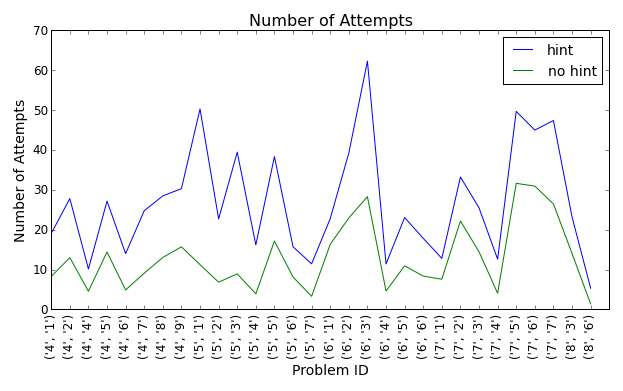
\includegraphics[width=0.5\textwidth]{image/tries_analysis.png} &
		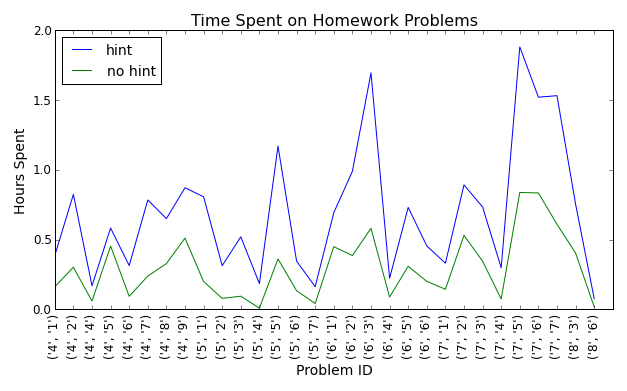
\includegraphics[width=0.5\textwidth]{image/times_analysis.png}
	\end{tabular}
    \label{fig:tries_times_analysis}
\end{figure}

Furthermore, we want to examine whether these two groups of students are significantly different. We perform a two-tailed t-test for both the average number of attempts and the average time spent on each problem. Our null hypothesis is that case students and control students have no difference on the average number of attempts and average time spent. We found that case students spent on average 16 more attempts than control students with a p-value $2.48*10^{-41}$. And case students spent on average 28 minutes more than control students with a p-value $6.63*10^{-36}$. We reject the hypothesis and conclude that control students and case students are significantly different. Case students who ask for hints are students who struggle with their homework. They spend more time and more attempts on these problems compared to control students.

Note that students who received hints are likely to spend more time on these problems because all our hints are short questions designed for students to answer. Students will likely to spend time to read and do the hint questions.

\subsection{Effect on Problems without Hint}
We then look at problems without hints. These are problems that neither case students nor control students receive any hints on. Our goal is to examine whether adaptive hints help students learn to solve similar problems when no hint is present.

For control students, we calculate average number of tries for each problem. Then, for each case student, we select problems that the student finished after receiving at least one hint. We filter out problems that the student finished before the first hint in each homework assignment and only look at problems that the student solved after seeing at least a hint. For example, the student solved an assignment of 9 problems in the following order $\{ 1, 4, 3, 2, 6, 5, 7, 8, 9\}$. This student received at least one hint on problem $\{3, 5, 7\}$. Therefore, we will only look at problem $\{2, 6, 8, 9\}$ in this assignment. See Figure. \ref{fig:pro_no_hint}. Then we compare the number of tries this case student spent with the average number of tries control students spent. Finally, we aggregate the differences of these four problems and consider it the difference of number of tries for this assignment between this case student and the control students. We repeat this process for every case student and at the end take the average of all case students.

\begin{figure}[ht]
   \centering
   \caption{We filter out the problems that come before the first problem with hints. We only look at problems that come after problem 3 in the above example. We then sum up the attempts and compare the sum of attempts for student A and our baseline.}
   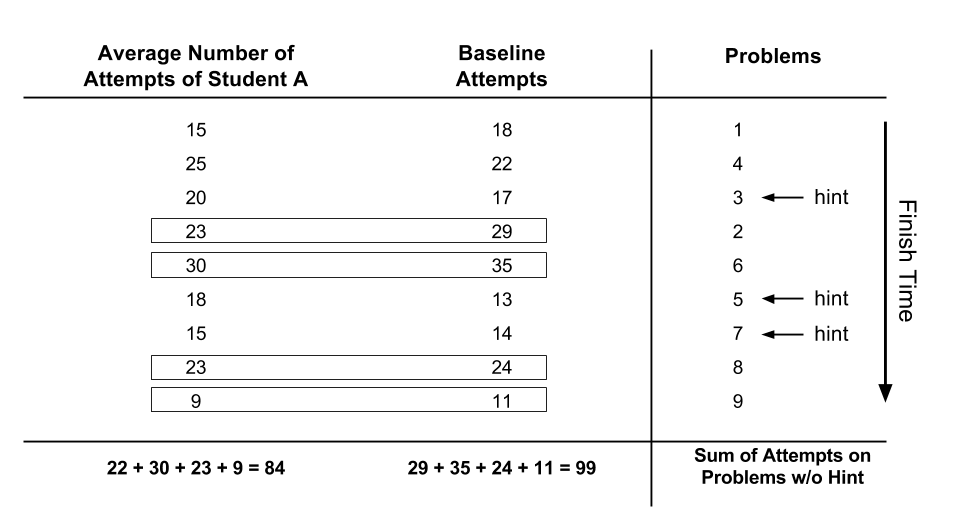
\includegraphics[width=0.8\textwidth]{image/Filter_problems.png}
   \label{fig:pro_no_hint}
\end{figure}


Our data shows that case students spend an average of 14.409 fewer attempts than the control students over all assignments. See Table \ref{tab:no_hint}. We again perform a two-tailed t-test. Our null hypothesis of our t-test is that case students have similar sum of attempts with control students. The p-value of our t-test is $2.9\%$. Therefore, we reject the null hypothesis and conclude that case students and control students have significantly different performance. This analysis shows that the adaptive hint system helps students to learn to solve similar problems that come later in the assignment. 

\begin{table}
\caption{The table listed the extra number of attempts that control students spent comparing to case students. We first compare the attempts for each assignment, then we look at all assignments at the end. We also perform a two tailed t-test with the null hypothesis that control students should have the same amount of attempts on problems as case students. The final p-value of the two tailed t-test for all assignments is small enough that we can reject the null hypothesis.}
\begin{center}
  \begin{tabular}{| c | c | c |}
  \hline
   Week & Average tries of & P-Value \\
      & control minus case  & \\ \hline
	4 & -1.051 & 0.829 \\
	5 & 14.559 & 0.00032 \\
	6 & 5.528 & 0.104 \\
	7 & 14.597 & 0.030 \\
	8 & -1.526 & 0.609 \\ \hline
    All Assignments & 14.409 & 0.029 \\ 
    \hline
  \end{tabular}
  \label{tab:no_hint}
  \end{center}
\end{table}

Table \ref{tab:no_hint} shows the differences of tries for each assignment. Assignment of week 4 and week 8 with very high p-value give negative results, but the results from week 5, 6, and 7 with very small p-value give positive results which lead to the positive result for all assignment. Further looking at week 4 data, we found that out of a total of 9 problems in week 4 assignment, problem 5 has 549 hints received and problem 9 has 96 hints received. The rest of the problems all have less than 50 hints received by students. This may cause the data to be too biased and therefore lead to a very large p-value. Also, Week 4 is the first week we send hints to students and students were in the process of learning how to request hints and how to learn from hints. Looking at week 8 in detail, we found that there are only 176 hints sent. Therefore, the data we collected for week 8 may not be enough for us to detect the difference between two groups of students.

We do similar analysis on the time students spend on problems. See Table \ref{tab:no_hint_time}. The results are consistent with our results of number of attempts. We have very consistent statistics that assignment 4 and assignment 8 have very high p-value comparing to the other assignments. The average of all assignments shows control students spent about 26 minutes more on each problem than case students.

\begin{table}
\caption{The table listed the extra seconds that control spent comparing to case. We first compare the time spent for each assignment, then we look at all assignments at the end. We perform a two tailed t-test with the null hypothesis that control students spent the same amount of time on problems as case students. The final p-value of the two tailed t-test for all assignments is small enough that we can reject the null hypothesis.}
\begin{center}
  \begin{tabular}{| c | c | c |}
  \hline
   Week & Average seconds of & P-Value \\
      & control minus case  & \\ \hline
	4 & -531.851 & 0.342 \\
	5 & 1116.101 & 0.00024 \\
	6 & 908.756 & 0.012 \\
	7 & 2324.41 & 0.006 \\
	8 & -208.903 & 0.507 \\ \hline
    All Assignments & 1573.682 & 0.012 \\ 
    \hline
  \end{tabular}
  \label{tab:no_hint_time}
  \end{center}
\end{table}

The statistics show us that the adaptive hints help students learn to solve problems and as a result improve students' performance in homework. Students who learn from hints perform better on similar problems comparing to students without hints.

\subsection{Effect on Final}
Final scores play an important role as to evaluate the learning outcome of students. We examine whether hints have effect on students' final score.

The problems in the final exam aim to examine students understanding of different topics learned throughout the college quarter. Each of these topics have a collection of homework problems for students to practice. Therefore, we select a set of homework problems for each of the final problem as shown in Table \ref{tab:map}.

\begin{table}[h]
\caption{Each final problem on the left has a set of corresponding homework problems on the right. The problem ID is in the format of week number and problem number. For example, (4,1) means problem 1 of week 4 assignment.}
\begin{center}
  \begin{tabular}{ c | c }
   Final Problem & Homework Problem IDs \\ \hline
	3 & (4,1), (4,2) \\
	4 & (5,1), (5,2), (5,3), (5,4) \\
    5 & (6,4) \\
    6 & (6,6) \\
    7 & (6,2), (6,3) \\
    8 & (8,3), (8,4), (8,5), (8,6) \\ \hline
  \end{tabular}
  \label{tab:map}
  \end{center}
\end{table}

For each final problem, we look at the corresponding assignment. The control and case students of the corresponding assignment will then be the control and case students of the final problem. We compare control and case students on their final score for each final problem. See Figure \ref{fig:final_compare_all}.

\begin{figure}[h]
\centering
\caption{The graph shows average final scores of each final problem. The data points are labeled with p-value of a two-tailed t-test. We don't see a very clear advantage on either of the control or case.}
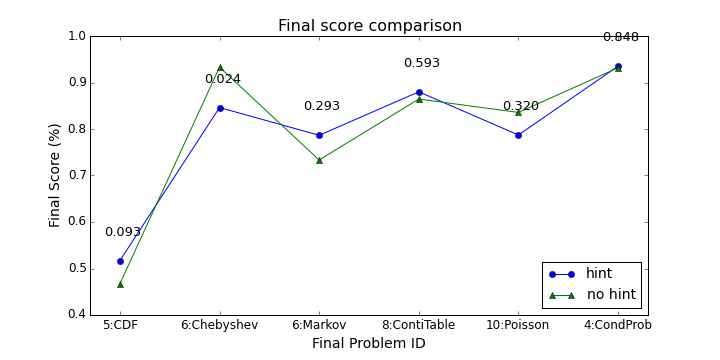
\includegraphics[width=0.8\linewidth, height=5cm]{image/final_compare.png}
\label{fig:final_compare_all}
\end{figure}

We can't tell which group of students perform better than the other. The p-values are not small enough and we conclude that the effect of hints on final scores is non-detectable.


\section{Conclusion}
We built an adaptive hint system for mathematics problems that can be embedded on any web-based homework platform. The system provides students with on-demand formative feedback to guide their learning process to achieve better learning outcome. Although we can't detect an improved learning outcome in the final exam, our statistics show an improvement of students' performance on homework. We show that students with the help of the adaptive hints spent less time and less try on homework problems compared to students without the help of hints.

\newpage
\bibliographystyle{splncs}
\bibliography{bibtxt}



\end{document}